\section{Études de l'impact des paramètres de l'algorithme FNC}
L'algorithme FNC est fonction de plusieurs paramètres ayant un impact à la fois sur les performances de décodage et sur
la complexité calculatoire. Cette section vise à étudier l'impact de chacun de ces paramètres sur les performances de 
décodage dans le cadre de turbo codes du standard LTE. Pour ce faire, une variation indépendante de chacun de ces 
paramètres est mené.

Tout d'abord, une première modification est effectuée vis-à-vis de l'algorithme \ref{alg:fc_b} présenté dans le chapitre
précédent. Maintenant, l'application de l'algorithme FNC n'est plus réalisé après la demi-itération dans le domaine
entrelacé mais après la demi-itération dans le domaine naturel. De la sorte, il n'est plus nécessaire d'effectuer une 
opération de désentrelacement avant de pouvoir calculer la vérification du CRC.

\subsection{Paramètres liés aux itérations}
Le premier groupe de paramètres correspond au choix des itérations du processus de turbo décodage sur lesquelles le 
principe FNC est appliqué. Il a été introduit dans le chapitre précédent que si l'itération minimale à partir de 
laquelle l'algorithme est trop faible, alors les performances de décodages peuvent être dégradées. Ceci dépend du risque 
d'erreur non détectée par le code détecteur d'erreurs. Cette probabilité est fonction de la taille de trame et de la 
taille du code CRC. En effet, pour une taille du code CRC constante, la probabilité d'erreur non détectée croît avec la
taille de la trame. 

Les Figures \ref{fig:fnc_min_528} à \ref{fig:fnc_min_6144} présentent l'impact de l'itération à partir de laquelle 
l'algorithme FNC commence à être applique (paramètre $I_\text{min}$) pour différents turbo codes du standard LTE. Dans 
ces trois cas, $I_\text{min}$ évolue de 2 à 8. Le nombre d'applications de l'algorithme FNC varie alors de 7 à 1. Il 
apparaît alors que pour chacun de ces codes, il existe une valeur optimale de $I_\text{min}$ au niveau des performances
de décodage. En dessous de cette valeur, la trop forte occurrence d'erreurs non détectées dégrade les performances de 
décodage, à tel point qu'elles peuvent être inférieures à celles d'un turbo décodeur conventionnel. Au delà de cette 
valeur optimale de $I_\text{min}$, à chaque fois que la valeur de $I_\text{min}$ est incrémentée, les performances
s'amenuisent légèrement.

\begin{figure}[!h]
	\centering
	\includegraphics[width=.9\textwidth,height=.5\textwidth]{main/ch4_fig/final/tikz_528/528_fnc10_minX.pdf}
	\caption{Performances de l'algorithme FNC pour K=528, $q=10$ et différentes valeurs de $I_\text{min}$. 
	Turbo décodeur basé sur l'algorithme EML-MAP itérant au plus 8 fois.
	\label{fig:fnc_min_528}}
\end{figure}

\begin{figure}[!h]
	\centering
	\includegraphics[width=.9\textwidth,height=.5\textwidth]{main/ch4_fig/final/tikz_2048/2048_fnc10_minX.pdf}
	\caption{Performances de l'algorithme FNC pour K=2048, $q=10$ et différentes valeurs de $I_\text{min}$. 
	Turbo décodeur basé sur l'algorithme EML-MAP itérant au plus 8 fois.
	\label{fig:fnc_min_2048}}
\end{figure}

\begin{figure}[!h]
	\centering 
	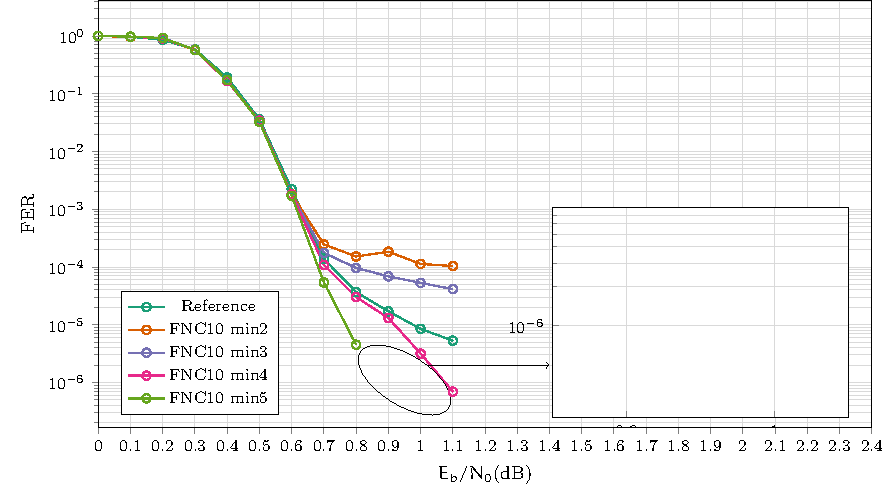
\includegraphics[width=.9\textwidth,height=.5\textwidth]{main/ch4_fig/final/tikz_6144/6144_fnc10_minX.pdf}
	\caption{Performances de l'algorithme FNC pour K=6144, $q=10$ et différentes valeurs de $I_\text{min}$. 
	Turbo décodeur basé sur l'algorithme EML-MAP itérant au plus 8 fois.
	\label{fig:fnc_min_6144}}
\end{figure}

Afin de dresser l'impact de chacune des itérations à laquelle l’algorithme FNC est appliqué, la Figure 
\ref{fig:fnc_only_2048} présente les performances de décodage avec une seule application de l'algorithme FNC pour le 
turbo code K=2048. Il apparaît alors que les performances sont équivalentes entre ces différents contextes. 
Une dégradation apparaît néanmoins vis-à-vis de la possibilité d'effectuer l'algorithme à toutes les itérations à partir
de l'itération $I_\text{min}$.

\begin{figure}[!h]
	\centering
	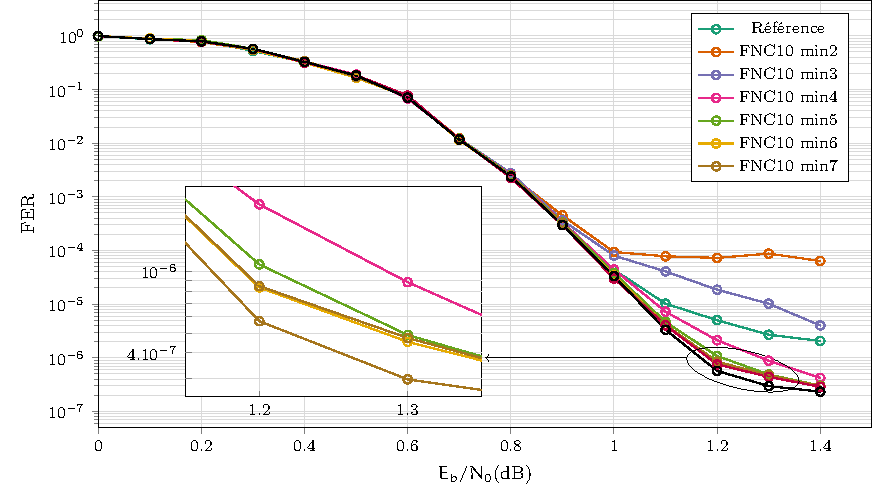
\includegraphics[width=.9\textwidth,height=.5\textwidth]{main/ch4_fig/final/tikz_2048/2048_fnc10_onlyX.pdf}
	\caption{Performances de l'algorithme FNC appliqué à une seule itération ($I_\text{FNC}$) pour K=2048, $q=10$.
	Turbo décodeur basé sur l'algorithme EML-MAP itérant au plus 8 fois.
	\label{fig:fnc_only_2048}}
\end{figure}

Finalement, il peut être intéressant de ne considérer l'application de l'algorithme uniquement toutes les deux 
itérations. Ceci permet alors d'obtenir une budget temps plus important pour effectuer l'algorithme FNC. La Figure 
\ref{fig:fnc_2048_s2} présente cet impact de la diminution par deux du nombre d'itérations sur les quelles l'algorithme FNC
est appliqué. À nouveau, des dégradations apparaissent mais elles sont moins conséquentes que dans le cas précédent.

\begin{figure}[!h]
	\centering
	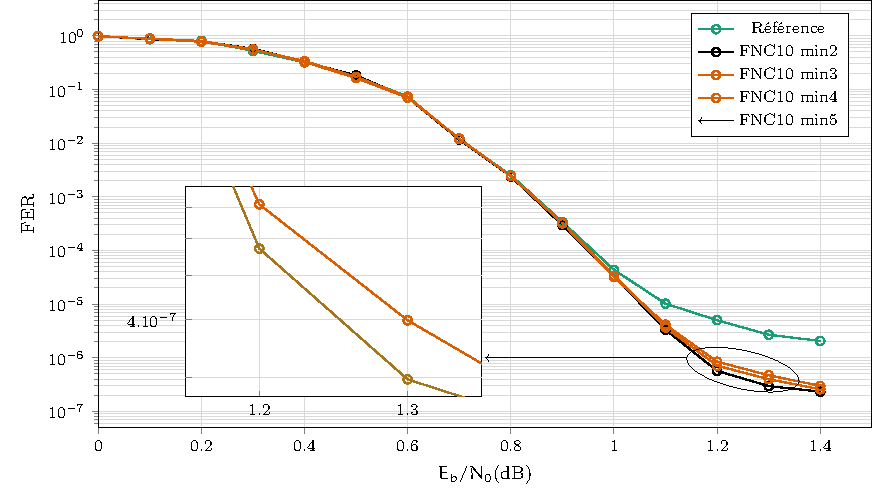
\includegraphics[width=.9\textwidth,height=.5\textwidth]{main/ch4_fig/final/tikz_2048/2048_fnc10_m5_s2.pdf}
	\caption{Performances de l'algorithme FNC appliqué toutes les deux itérations ($I_\text{FNC}$) pour K=2048, $q=10$.
	Turbo décodeur basé sur l'algorithme EML-MAP itérant au plus 8 fois.
	\label{fig:fnc_2048_s2}}
\end{figure}

En conclusion de cette étude, une trop faible valeur de $I_\text{min}$ est néfaste aux performances de l'algorithme. 
La valeur optimale de $I_\text{min}$ en terme de performances de décodages résultantes est entièrement dépendante des
capacités de détection du code détecteur d'erreur. L'application de l'algorithme FNC après chaque itération de turbo 
décodage permet d'obtenir les meilleures performances de décodage. Chaque suppression d'application du principe FNC 
dégrade les performances optimales. Néanmoins, ne pas appliquer à chaque itération l'algorithme permet d'augmenter le 
budget temps pour le traitement de cet algorithme et permettra donc de réduire la complexité matérielle de 
l'implémentation de l'algorithme FNC. Ceci sera détaillé dans une section prochaine de ce chapitre.

Maintenant, l'étude de l'impact de la valeur de $q$, correspondant à la profondeur de recherche, est mené.

\subsection{Impact de la taille de recherche}
Il a été présenté dans le chapitre précédent que les performances de l'algorithme FNC était très fortement conditionnées
par la taille du vecteur de recherche de positions probablement erronées $q$. En effet, incrémenter $q$ de $1$ revient 
à considérer deux fois plus de mots candidats. Ceci augmente de fait la probabilité d'identifier le bon mot de code. 
Cependant, la complexité calculatoire se voit donc doublée pour chaque incrément de $q$. 

Les Figures \ref{fig:fnc_min_528_q} à \ref{fig:fnc_min_6144_q} présentent l'impact de l'évolution de la valeur de $q$ 
pour les turbo codes du standard LTE pour une taille de trame allant de K=528 à K=6144. Dans tous les cas, l'algorithme 
FNC est utilisé toutes les itérations à partir de l'itération $I_\text{min}$ telles que les performances de décodages 
soient les meilleures pour $q=10$. Dans l'ensemble, comme attendu, il apparaît que la réduction de $q$ impacte 
négativement les performances de décodage. Cependant, cet impact dépend du turbo ode considéré. Par exemple, pour 
$K=528$, le passage de $q=10$ à $q=8$ a un impact plus défavorable que le passage de $q=8$ à $q=6$. Ceci s'explique par
la distribution des erreurs binaires de ce turbo code. En effet, une part non négligeable des trames erronées contiennent
9 erreurs (cf. Figure \ref{fig:be}). Elles ne peuvent donc être corrigées seulement dans les cas tels que $q\geq 9$. En 
revanche, pour $K=2048$, la très grande majorité des trames erronées contiennent strictement moins de 6 erreurs binaires.
Ceci explique la similitude des performances de décodage pour une valeur de $q$ comprise entre 10 et 6. En revanche, le 
passage de q=6 à q=4 impacte plus négativement les performances de décodage de l'algorithme FNC.  

\begin{figure}[!h]
	\centering
	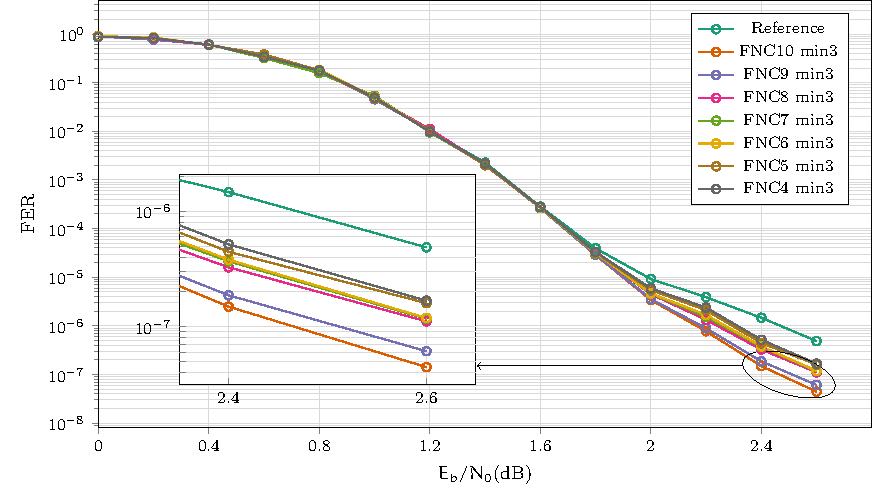
\includegraphics[width=.9\textwidth,height=.5\textwidth]{main/ch4_fig/final/tikz_528/528_fncX_min3.pdf}
	\caption{Performances de l'algorithme FNC pour K=528 et différentes valeurs de $q$. 
	Turbo décodeur basé sur l'algorithme EML-MAP itérant au plus 8 fois.
	\label{fig:fnc_min_528_q}}
\end{figure}

\begin{figure}[!h]
	\centering
	\includegraphics[width=.9\textwidth,height=.5\textwidth]{main/ch4_fig/final/tikz_2048/2048_fncX_min5.pdf}
	\caption{Performances de l'algorithme FNC pour K=2048 et différentes valeurs de $q$..  
	Turbo décodeur basé sur l'algorithme EML-MAP itérant au plus 8 fois. 
	\label{fig:fnc_min_2048_q}}
\end{figure}

\begin{figure}[!h]
	\centering
	\includegraphics[width=.9\textwidth,height=.5\textwidth, draft]{main/ch4_fig/final/tikz_6144/6144_fncX_min5.pdf}
	\caption{Performances de l'algorithme FNC pour K=6144 et différentes valeurs de $q$.
	Turbo décodeur basé sur l'algorithme EML-MAP itérant au plus 8 fois.
	\label{fig:fnc_min_6144_q}}
\end{figure}

Finalement il apparaît que la valeur de $q$ proposant le meilleur ratio entre amélioration des performances de décodage 
dépend fortement du turbo code considéré. Néanmoins, puisque les valeurs de $q$ supérieurs à 10 n'apportent qu'un gain 
marginal sur les performances de décodage, il est opportun de ne pas considérer de valeurs supérieures. Ceci serait à 
nuancer dans le contexte d'un autre standard considérant un code CRC possédant de meilleures propriétés de distance.

Le dernier vecteur de modifications de l'algorithme FNC pour son implémentation concerne la représentation de 
l'information en virgule fixe. Ceci est l'objet de la prochaine section.


\subsection{L'algorithme FNC et la quantification de l'information}
Dans un premier temps, il est nécessaire de vérifier que l'algorithme FNC supporte un passage en virgule fixe.
Les résultats sont présentés en Figure \ref{fig:fnc_fp}; Dans ce cas, toutes les données internes du turbo 
décodeur ont une dynamique inférieure à 8 bits. Des étapes de normalisation internes au processus itératif sont 
réalisées afin de fournir des performances de décodages proches de celles d'un décodeur utilisant une représentation 
flottante de l'information. Sur cette Figure, il apparaît que la dégradation induite par le passage en représentation à 
virgule fixe sur 8 bits est la même que le décodeur utilise ou non le principe FNC. Ainsi, les gains en performance de 
décodage sont conservés malgré le changement de représentation de l'information.

\begin{figure}[!h]
	\centering
	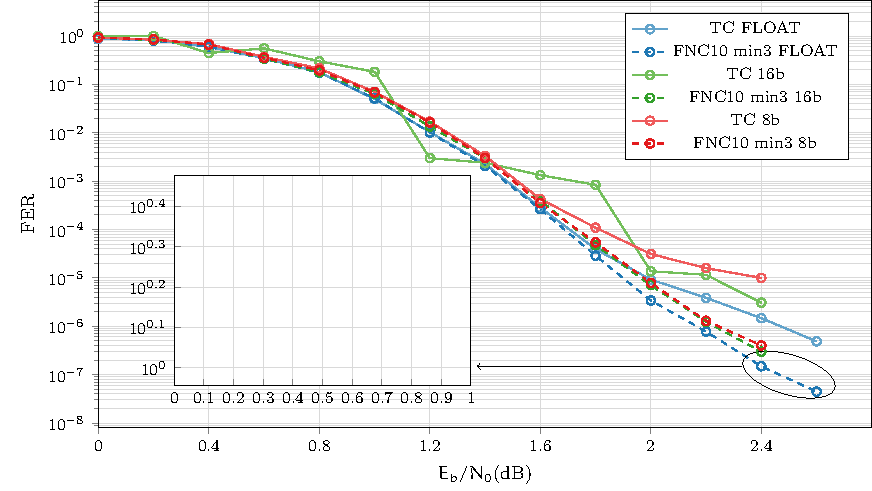
\includegraphics[width=.9\textwidth,height=.5\textwidth]{main/ch4_fig/final/tikz_prec/528_refs_prec.pdf}
	\caption{Comparaison des performances de l'algorithme FNC pour K=528 et $q=10$ suivant la représentation de 
	l'information utilisée.
	Turbo décodeur basé sur l'algorithme EML-MAP itérant au plus 8 fois.
	\label{fig:fnc_fp}}
\end{figure}

Dans ce contexte, comme la métrique $\Delta$ est basée sur la valeur absolue d'une somme, sa dynamique reste  sur 
8 bits. Or, ce sont les valeurs minimales de la métrique $\Delta$ qui sont exploitées par l'algorithme FNC. La Figure 
\ref{fig:fnc_fp_b} présente l'impact d'une saturation sur les éléments de la métrique $\Delta$ avant son utilisation par 
l'algorithme FNC. Le nombre de bits utilisés pour la métrique $\Delta$, noté $b_{\Delta}$ varie alors de 8 à 3. La 
valeur de $q$ est fixée à 10 et K vaut 528. Il apparaît alors que  \\
TODO\\TODO\\TODO

\begin{figure}[!h]
	\centering
	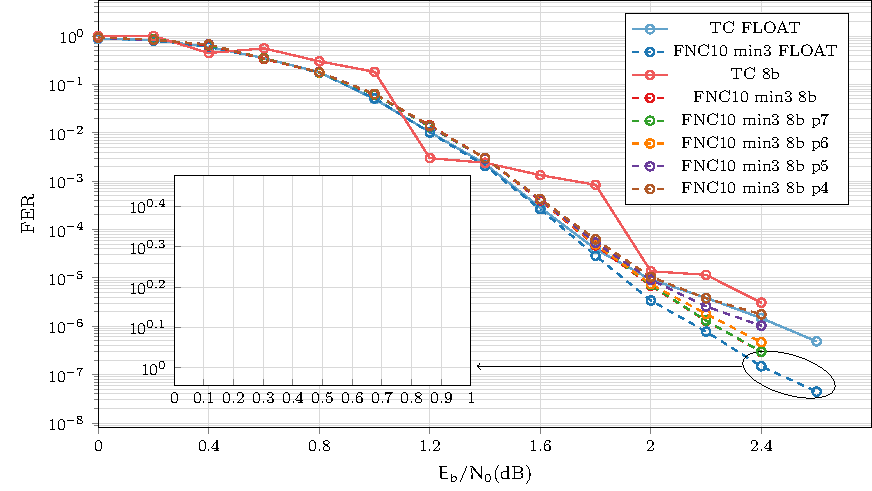
\includegraphics[width=.9\textwidth,height=.5\textwidth]{main/ch4_fig/final/tikz_prec/528_16b.pdf}
	\caption{Performances de l'algorithme FNC pour K=528 et $q=10$ en fonction de la dynamique de la métrique $\Delta$.
	Turbo décodeur basé sur l'algorithme EML-MAP itérant au plus 8 fois.
	\label{fig:fnc_fp_16b}}
\end{figure}

\begin{figure}[!h]
	\centering
	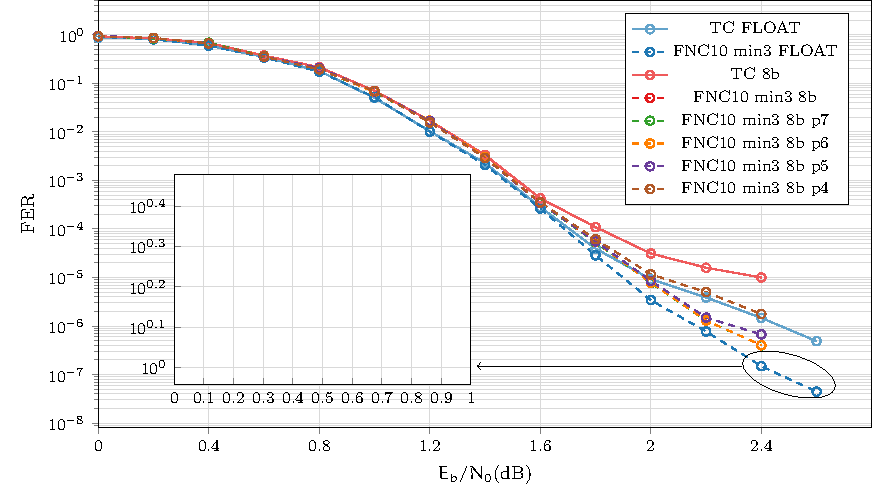
\includegraphics[width=.9\textwidth,height=.5\textwidth]{main/ch4_fig/final/tikz_prec/528_8b.pdf}
	\caption{Performances de l'algorithme FNC pour K=528 et $q=10$ en fonction de la dynamique de la métrique $\Delta$.
	Turbo décodeur basé sur l'algorithme EML-MAP itérant au plus 8 fois.
	\label{fig:fnc_fp_8b}}
\end{figure}

En conclusion, pour un turbo décodeur utilisant 8 bits pour ces métriques internes, fixer la valeur de $b_{\Delta}$ 
permet de limiter la dynamique des données en entrée de l'algorithme FNC tout en fournissant les mêmes performances de
décodage sans saturation.

\subsection{Conclusion}
Dans cette section, une étude de l'impact des différents paramètres de l'algorithme FNC a été menée. Ces paramètres ont
pour la plupart un impact sur les performances de décodage et la complexité calculatoire de l'algorithme FNC. Suivant 
les performances de décodage visées et l'ajout de complexité calculatoire toléré, le concepteur d'un turbo décodeur 
utilisant l'algorithme FNC devra choisir les valeurs de ces différents paramètres en conséquence.

La section suivante présente une architecture matérielle pour l'algorithme FNC dans le contexte d'un turbo décodeur 
séquentiel basé sur l'ordonnancement Backward-Forward-Sliding-Window. L'impact sur la complexité matérielle des 
paramètres précédents sera alors étudiée.